\resizebox{\textwidth}{!}{%
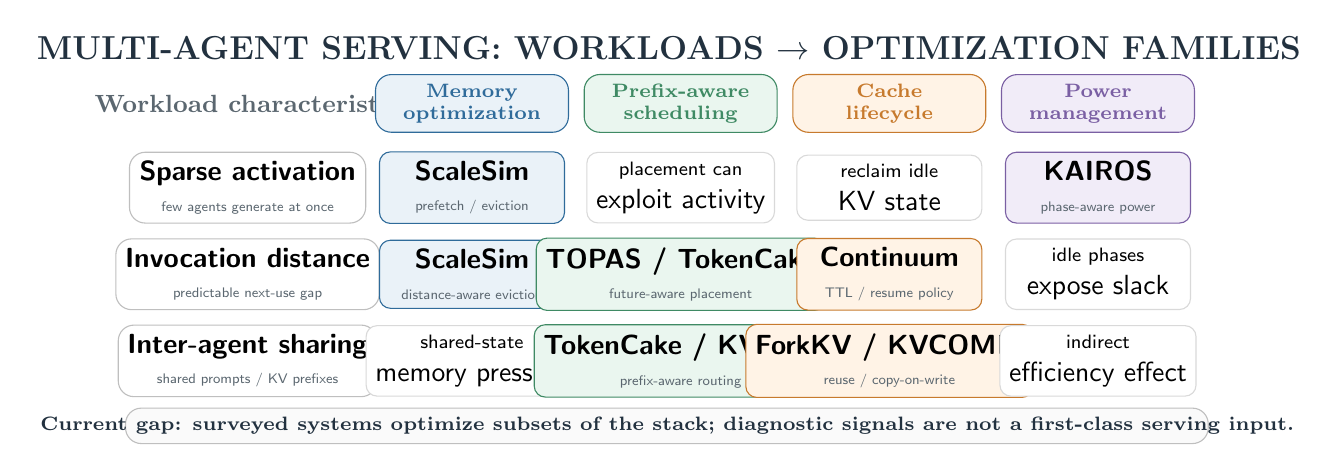
\begin{tikzpicture}[x=1cm,y=1cm,font=\sffamily]
\definecolor{cblue}{HTML}{2F6B9A}\definecolor{cbluel}{HTML}{EAF2F8}
\definecolor{cgreen}{HTML}{3F8A64}\definecolor{cgreenl}{HTML}{EAF6EF}
\definecolor{corange}{HTML}{C77A2D}\definecolor{corangel}{HTML}{FFF3E6}
\definecolor{cpurple}{HTML}{7A5FA3}\definecolor{cpurplel}{HTML}{F1ECF8}
\definecolor{cdark}{HTML}{22313F}\definecolor{cmid}{HTML}{5B6770}
\tikzset{rowbox/.style={rounded corners=2mm,draw=black!25,fill=white,minimum width=3.0cm,minimum height=0.82cm,align=center},
 cell/.style={rounded corners=1.4mm,draw=black!15,fill=white,minimum width=2.35cm,minimum height=0.82cm,align=center}}
\node[font=\bfseries\large,text=cdark] at (7,5.05) {MULTI-AGENT SERVING: WORKLOADS $\rightarrow$ OPTIMIZATION FAMILIES};
\node[font=\bfseries\small,text=cmid] at (1.65,4.35) {Workload characteristic};
\node[rounded corners=2mm,draw=cblue,fill=cbluel,minimum width=2.45cm,minimum height=0.72cm,align=center,font=\bfseries\scriptsize,text=cblue] at (4.50,4.35) {Memory\\optimization};
\node[rounded corners=2mm,draw=cgreen,fill=cgreenl,minimum width=2.45cm,minimum height=0.72cm,align=center,font=\bfseries\scriptsize,text=cgreen] at (7.15,4.35) {Prefix-aware\\scheduling};
\node[rounded corners=2mm,draw=corange,fill=corangel,minimum width=2.45cm,minimum height=0.72cm,align=center,font=\bfseries\scriptsize,text=corange] at (9.80,4.35) {Cache\\lifecycle};
\node[rounded corners=2mm,draw=cpurple,fill=cpurplel,minimum width=2.45cm,minimum height=0.72cm,align=center,font=\bfseries\scriptsize,text=cpurple] at (12.45,4.35) {Power\\management};
\node[rowbox] at (1.65,3.28) {\bfseries Sparse activation\\[-1pt]\tiny\color{cmid}few agents generate at once};
\node[cell,draw=cblue,fill=cbluel] at (4.50,3.28) {\bfseries ScaleSim\\[-1pt]\tiny\color{cmid}prefetch / eviction};
\node[cell] at (7.15,3.28) {\scriptsize placement can\\exploit activity};
\node[cell] at (9.80,3.28) {\scriptsize reclaim idle\\KV state};
\node[cell,draw=cpurple,fill=cpurplel] at (12.45,3.28) {\bfseries KAIROS\\[-1pt]\tiny\color{cmid}phase-aware power};
\node[rowbox] at (1.65,2.18) {\bfseries Invocation distance\\[-1pt]\tiny\color{cmid}predictable next-use gap};
\node[cell,draw=cblue,fill=cbluel] at (4.50,2.18) {\bfseries ScaleSim\\[-1pt]\tiny\color{cmid}distance-aware eviction};
\node[cell,draw=cgreen,fill=cgreenl] at (7.15,2.18) {\bfseries TOPAS / TokenCake\\[-1pt]\tiny\color{cmid}future-aware placement};
\node[cell,draw=corange,fill=corangel] at (9.80,2.18) {\bfseries Continuum\\[-1pt]\tiny\color{cmid}TTL / resume policy};
\node[cell] at (12.45,2.18) {\scriptsize idle phases\\expose slack};
\node[rowbox] at (1.65,1.08) {\bfseries Inter-agent sharing\\[-1pt]\tiny\color{cmid}shared prompts / KV prefixes};
\node[cell] at (4.50,1.08) {\scriptsize shared-state\\memory pressure};
\node[cell,draw=cgreen,fill=cgreenl] at (7.15,1.08) {\bfseries TokenCake / KVFlow\\[-1pt]\tiny\color{cmid}prefix-aware routing};
\node[cell,draw=corange,fill=corangel] at (9.80,1.08) {\bfseries ForkKV / KVCOMM\\[-1pt]\tiny\color{cmid}reuse / copy-on-write};
\node[cell] at (12.45,1.08) {\scriptsize indirect\\efficiency effect};
\draw[rounded corners=2mm,draw=black!25,fill=black!2] (0.1,0.03) rectangle (13.85,0.48);
\node[font=\scriptsize,text=cdark,align=center] at (6.98,0.255) {\bfseries Current gap: surveyed systems optimize subsets of the stack; diagnostic signals are not a first-class serving input.};
\end{tikzpicture}%
}
